\documentclass[a4paper]{article}

\usepackage[pages=all, color=black, position={current page.south}, placement=bottom, scale=1, opacity=1, vshift=5mm]{background}
\usepackage[margin=1in]{geometry} % full-width
\backgroundsetup{
  contents={},
  color=black,
  opacity=1,
  position=current page.south,
  vshift=5mm
}

% AMS Packages
\usepackage{amsmath}
\usepackage{amsthm}
\usepackage{amssymb}

% Unicode
\usepackage[utf8]{inputenc}
\usepackage[colorlinks=true,allcolors=blue]{hyperref}
\hypersetup{
	unicode,
%	colorlinks,
%	breaklinks,
%	urlcolor=cyan, 
%	linkcolor=blue, 
	pdfauthor={Author One, Author Two, Author Three},
	pdftitle={A simple article template},
	pdfsubject={A simple article template},
	pdfkeywords={article, template, simple},
	pdfproducer={LaTeX},
	pdfcreator={pdflatex}
}

% Vietnamese
%\usepackage{vntex}

% Natbib
\usepackage[sort&compress,numbers,square]{natbib}
\usepackage{url}
\usepackage{hyperref}
\bibliographystyle{mplainnat}

% Theorem, Lemma, etc
\theoremstyle{plain}
\newtheorem{theorem}{Theorem}
\newtheorem{corollary}[theorem]{Corollary}
\newtheorem{lemma}[theorem]{Lemma}
\newtheorem{claim}{Claim}[theorem]
\newtheorem{axiom}[theorem]{Axiom}
\newtheorem{conjecture}[theorem]{Conjecture}
\newtheorem{fact}[theorem]{Fact}
\newtheorem{hypothesis}[theorem]{Hypothesis}
\newtheorem{assumption}[theorem]{Assumption}
\newtheorem{proposition}[theorem]{Proposition}
\newtheorem{criterion}[theorem]{Criterion}
\theoremstyle{definition}
\newtheorem{definition}[theorem]{Definition}
\newtheorem{example}[theorem]{Example}
\newtheorem{remark}[theorem]{Remark}
\newtheorem{problem}[theorem]{Problem}
\newtheorem{principle}[theorem]{Principle}
\usepackage{subcaption}
\usepackage{float}
% \usepackage{graphicx, color}IEEE
\graphicspath{{fig/}}

%\usepackage[linesnumbered,ruled,vlined,commentsnumbered]{algorithm2e} % use algorithm2e for typesetting algorithms
\usepackage{algorithm, algpseudocode} % use algorithm and algorithmicx for typesetting algorithms
\usepackage{mathrsfs} % for \mathscr command

\usepackage{lipsum}
\usepackage{booktabs} 

% Author info
\title{A Comprehensive Overlook on Employing Classical Machine Learning in Content Based Image Retrieval}
\author{Shyam Sathvik $^1$ \and Neermita Bhattacharya $^2$ \and Siddhesh Ayyathan  $^3$ \and Gubbala Bhargavi$^4$ \and Sakshi Sharma $^5$  }

\date{
	$^1$Indian Institute of Technology, Jodhpur, Jodhpur 342037, India \\ \texttt{\{b22ee036, b22cs092, b22cs016, b22cs022, b22cs073\}@iitj.ac.in}\\%
	% $^2$Organization 2 \\ \texttt{auth3@inst2.edu}\\[2ex]%
%	\today
}


\begin{document}
	\maketitle
	
	\begin{abstract}
		\noindent Image Retrieval task on every possible permutation of images while only using Classical Machine Learning tasks is a challenging task. Our project's scope is limited to the CIFAR-10 dataset, which contains 10 distinguishable classes. 
        \begin{figure}
            \centering
            \includegraphics[width=0.77\linewidth]{Figures/Classes.png}
            \caption{The different classes present in CIFAR-10}
            \label{fig:enter-label}
        \end{figure}
    % Image of CIFAR 10 Dataset will be inserted here 
    We aim to lay down the different machine learning techniques followed, the details of the performed experiments, the details of programmatic implementations of the algorithms the team has come up with, and the results of the implementation, along with failure case analysis.
    
    \noindent 
    Literature review and examination of SOTA performance on CIFAR10 has shown that the best-performing models are a result of advanced Computer Vision techniques, Convolutional Neural Networks, and other advanced Neural Network Architectures. These advanced methods yield extremely high performance. Limited to Classical Machine Learning Techniques, we tackle this task by adhering to the first principles.

    \noindent 
    Dimensionality reduction techniques such as Principal Component Analysis (PCA), Histogram of Oriented Gradients (HOG), Scale-Invariant Feature Transform (SIFT), and Linear Discriminant Analysis (LDA) over various powerful classifiers namely K-nearest neighbors, Decision Trees, Random Forests, AdaBoost, and SVM were implemented on images from the CIFAR-10 dataset. We also apply a clustering-based model (K-Means) as part of our image retrieval system and Artificial Neural Networks using Fourier Domain analysis.

    
    
		\vspace{10cm}	
		% \noindent\textbf{Keywords:} article, template, simple
	\end{abstract}

\tableofcontents
\newpage
\section{Problem Setting}
\label{sec:intro}
\subsection {Introduction}
\noindent With the rapid development of computer technology, the amount of digital imagery data has been rapidly increasing. There is an inevitable need for efficient systems that help retrieve visual information aligning with the user's interest since image retrieval plays a major role in an integrated healthcare environment for various purposes, such as computer-aided diagnosis, medical education, tele-surgery, and evidence-based medicine. From diagnosing medical conditions to monitoring environmental changes, image retrieval systems play a vital role in solving real-world problems and advancing scientific research.
\newline

\noindent This paper deals with developing a satisfactory Image Retrieval System using traditional Machine Learning techniques, abstaining from the usage of modern technologies like Computer Vision and Deep Learning. We also assess the performances of various classical models coupled with feature extraction techniques. We discuss the performance of Classification and Clustering models, along with a light usage of ANNs and Similarity Functions. %edit this
\newline
        
% \noindent Upon employing multiple feature extraction techniques and different classifiers, we have observed that Histogram of Oriented Gradients (HOG) along with SVM and Random Forests obtained an accuracy of over 50\%, outperforming other methods. Applying SIFT as a feature extractor resulted in extremely poor models having a accuracy of just 10\%. 
    

\noindent Furthermore, our research delves into the utilization of Fast Fourier Transform with Artificial Neural Networks (ANNs). By harnessing the frequency domain representations provided by FFT, coupled with the learning capabilities of ANNs, we aim to explore novel approaches for image analysis and feature extraction, potentially uncovering latent patterns and correlations within the data.\%.
\newline
    
\noindent Performances of clustering models using K-Means with Principal Component Analysis, Linear Discriminant Analysis, and t-distributed Stochastic Neighbor Embedding have been reported too. The t-SNE dimensionality reduction technique is shown to display clear and concise clusters while the former techniques exhibit plenty of overlap. 
% This paragraph will also contain results related to clustering . 
\newline
    
\noindent Through this comprehensive investigation, we aim to provide insights into the comparative effectiveness, strengths, and limitations of different dimensionality reduction techniques, classification algorithms, and clustering models in the domain of image analysis. 
\newline

\noindent The sections ahead in this paper discuss the existing literature and SOTA algorithms for image classification, the approaches tried by our team, the experiments and results obtained, a concise summary including failure case analysis, and the contribution of each member.

\newpage
        
	
\subsection{Literature Review}
	% This is how you cite~\cite{cstbir2024aaai}. Please keep all bib entries in ref.bib.
 % \newline
\noindent With the onset of this project, papers{~\cite{belhi2020cnn} and}{~\cite{datta2008image}  were referred to initially. We discuss the main papers our team focused on in this section.\newline
\noindent 

\noindent\textbf{~\cite{guo2002learning} Paper Review 1}\newline

\noindent\textbf{Title: "Learning Similarity Measure for Natural Image Retrieval With Relevance Feedback."}
\newline
%  make sure the link is working 
\href {https://ieeexplore.ieee.org/stamp/stamp.jsp?tp=&arnumber=1021882&tag=1}{IEEE Xplore} \newline
The paper provides an overview of content-based image retrieval approaches, focusing on classical
machine learning techniques applied in image-based retrieval systems. It discusses various
methodologies and trends shaping the field of CBIR, with an emphasis on feature-based and semantics-based retrieval techniques. \newline

\noindent \textit {Key Machine Learning Techniques}:
\newline

The paper discusses several key machine learning techniques that include:
1. Feature-based Methods: These methods involve the extraction of low-level visual features such as color, texture, and shape from images. Classical machine learning algorithms like k-nearest neighbors (KNN), support vector machines (SVM), and decision trees are commonly used
for similarity measurement and classification based on these extracted features.
2. By utilizing these machine learning algorithms, the system learns a boundary that filters
images for similarity measures.
3. Perhaps the most important aspect of this paper is the Constrained Similarity Measure approach. The CSM is a method used for image retrieval that integrates boundary learning techniques such as AdaBoost and SVM. After learning a boundary based on user feedback, images
are filtered based on their relationship to this boundary. Images inside the boundary are ranked by their Euclidean distances to the query. For images outside the boundary, a distance-from-boundary (DFB) measure is utilized to rank them. This ensures that potentially similar images, which may not be enclosed by the boundary, are not overlooked during retrieval, thereby providing a more comprehensive set of results to the user. \newline

\noindent \textit {Performance:}
\newline

The study evaluates the constrained similarity measure using a subset of the Corel photo Gallery
image database, consisting of 10,009 images categorized into 79 concepts. Precision and recall
are employed to assess retrieval performance, with feedback from users aiding in refinement.
Results demonstrate that CSM significantly improves both precision and recall, particularly after
one or two iterations of feedback. Additionally, boundary learning with Support Vector Machines
(SVM) consistently outperforms AdaBoost in most cases, showcasing the effectiveness of SVM-based
CSM. Precision initially rises with feedback for CSM, offering users a larger pool of similar
images early on, but gradually declines while still surpassing Euclidean distance-based
retrieval.
\newline
\newpage
\noindent\textbf{\cite{hertz2004learning} Paper Review 2} \newline
        
\noindent\textbf{Title: "Learning Distance Functions for Image Retrieval"}
\newline
%  make sure the link is working 
\href {https://ieeexplore.ieee.org/stamp/stamp.jsp?tp=&arnumber=1315215&tag=1}{IEEE Xplore} \newline
This paper proposes a novel approach to image retrieval by learning distance functions using binary classifiers with margins. The classifiers are trained on pairs of images, distinguishing between pairs from the same class and pairs from different classes, with the signed margin serving as the distance function. The authors investigate various variants of this approach,
employing SVM and Boosting algorithms as product space classifiers. \newline

\noindent \textit {Key Machine Learning Techniques}:
\newline

1. Binary classifiers with margins: These classifiers are trained to distinguish between pairs in
which the images are from the same class and pairs containing images from different classes.
2. Boosting: Boosting algorithms are employed to combine multiple weak learners sequentially to
improve classification performance. In this context, boosting is utilized over the product
space to enhance the binary classifiers' performance.
3. Constrained EM algorithm: The weak learner used in the boosting scheme is based on a constrained Expectation-Maximization (EM) algorithm. This algorithm computes a Gaussian mixture model, providing a partition of the original feature space while adhering to equivalence constraints.
4. Margin-based distance learning: The authors focus on margin-based distance learning methods, which aim to learn distance functions that optimize margins between classes. This contrasts with traditional metric learning approaches, such as learning Mahalanobis distances.\newline

\noindent \textit {Performance:} \newline

The proposed techniques are evaluated on various benchmark datasets, including those from the UCI
repository, the YaleB facial image dataset, and a dataset of natural images from a commercial image CD. DistBoost achieves significant improvements over Mahalanobis based distance measures (in neighbor purity plots) and also outperforms all other product space learning methods.
Using a subset of the YaleB facial image database, the images (a total of 1920 images, including 64 frontal pose images of 30 different subjects) were centered using optical flow. They were then converted to vectors, and each image was represented using its first 60 PCA coefficients.
We notice that the performance of SVM and C4.5Boost severely degrades, indicating strong overfit behavior. The DistBoost, on the other hand, degrades gracefully and is still better than the other alternatives.


 
\newpage
	
	
	\section{Our Approaches}
	\label{sec:app}
 \subsection{Dataset description}
The dataset used is the CIFAR-10 dataset by Alex Krizhevsky, Vinod Nair, and Geoffrey Hinton. It comprises 60,000 color images, each with a resolution of 32x32 pixels, distributed across 10 classes. These classes represent various objects and animals commonly found in everyday life. The dataset encompasses a diverse range of objects and animals, including:
Airplane, Automobile, Bird, Cat, Deer, Dog, Frog, Horse, Ship, and Truck.
\newline

\noindent Training and Test Sets:
The training set contains 50,000 images (5,000 images per class) used for model training.
The test set contains 10,000 images (1,000 images per class) used for evaluating model performance. Each image has a size (1, 32, 32, 3) with 3 RGB channels. The training and test dataset shapes are given below:
\newline

\begin{table}[H]
    \centering
    \caption{Data Shape}
    \begin{tabular}{lcccc}
        \hline
        Type & Shape \\
        \hline
        Train data & (50000, 32, 32, 3) \\
        Train labels & (50000, 1) \\
        Test data & (10000, 32, 32, 3) \\
        Test labels & (10000, 1) \\
        \hline
    \end{tabular}
\end{table}

\noindent \newline Images in the dataset exhibit variations in lighting conditions, backgrounds, and viewpoints to make classification tasks non-trivial. 
The resolution of each of the images is extremely low (32x32 pixels). 
For feature extraction, each of the images was first flattened to vectors of size (1, 3072). 




We now discuss each of these techniques in detail.
% \newpage

\subsection {Feature Extraction Techniques Employed}

\noindent Feature Extraction is an important aspect of building efficient machine learning models. They can improve the performance of the models if chosen and used appropriately. Since we're dealing with images in this work, the flattened vectors used for training the models are usually svery big and often contain a lot of unecessary data, such as the pixel values of the background, hence, obstructing the model from localizing on to the object in the image in question. Therefore, it becomes imperative that we choose appropriate feature extraction and dimensionality reduction techniques to both save time and power in training while ensuring the quality of the feature vectors we're working with. Keeping the above in mind, we pick the following feature extraction techniques to use for this project: 

\begin{itemize}
  \item Principal Component Analysis (PCA)
  \item Linear Discriminant Analysis (LDA)
  \item Histogram of Oriented Gradients (HOG)
  \item Scale-Invariant Feature Transform (SIFT)
   \item t-distributed Stochastic Neighbor Embedding (t-SNE)
  % \item Using convolutions in the Fourier Domain
  \item Pre-trained Convolutional Neural Networks (VGG/ResNet)
\end{itemize}

\noindent We now discuss each of the techniques employed in brief and how they add value to the learning.

\subsubsection{PCA}
\begin{itemize}
    \item[] \textbf{Dimensionality Reduction:} PCA is primarily used for reducing the dimensionality of high-dimensional datasets while retaining most of the variability present in the data.
    
    \item[] \textbf{Orthogonal Transformation:} PCA transforms the original features into a new set of orthogonal features called principal components. These components are ordered in terms of the amount of variance they explain in the data.
    
    \item[] \textbf{Variance Maximization:} The first principal component captures the maximum variance in the data, followed by subsequent components, each capturing orthogonal variance unexplained by the previous components. A plot between the number of components and the cumulative explained variance ratio displays the best range of components needed to retrieve the maximum data.
    
    \item[] \textbf{Linear Transformation:} PCA performs a linear transformation on the data by projecting it onto a lower-dimensional subspace spanned by the principal components. The principal components can be computed by eigenvalue decomposition of the covariance matrix of the data. The topmost eigenvalues and their corresponding eigenvectors are chosen.

\end{itemize}

\subsubsection{SIFT}
\begin{itemize}
    \item[] \textbf{Robustness:} SIFT is robust to scale, rotation, and illumination changes.
    
    \item[] \textbf{Keypoint Detection:} It identifies keypoints and computes descriptors based on local gradient orientations.
    
    \item[] \textbf{Scaling Invariance:} SIFT features are invariant to scaling.
    
    \item[] \textbf{Visual Similarity Retrieval:} It also facilitates image retrieval based on visual similarity.
\end{itemize}
\subsubsection{LDA}

\begin{itemize}
    \item[] \textbf{Enhancing Discriminative Power:} LDA is a dimensionality reduction technique aimed at enhancing the discriminative power of feature vectors.
    
    \item[] \textbf{Maximizing Class Separation:} By projecting feature vectors onto a lower-dimensional space, LDA maximizes class separation. LDA focuses on maximising the distance between two different classes while minimizing the spread within the classes themselves.
    
    \item[] \textbf{Reducing Computational Complexity:} LDA reduces computational complexity while preserving relevant discriminative information.
    
    \item[] \textbf{Improving Similarity Measurement:} In image retrieval, LDA improves the effectiveness of similarity measurement.
    
    \item[] \textbf{Efficient Retrieval:} LDA facilitates efficient retrieval by reducing feature dimensionality without compromising relevance.
\end{itemize}
\subsubsection {HOG}
\begin{itemize}
    \item[] \textbf{Histogram Computation:} HOG computes histograms of gradient orientations within spatial regions of an image. It analyzes the distribution of edge orientations within an object to describe its shape and appearance. 
    
    \item[] \textbf{Shape and Structure Representation:} HOG captures shape information and local structure of objects, making it effective for object detection and recognition. It involves computing the gradient magnitude and orientation for each pixel in an image and then dividing the image into small cells.
    
    \item[] \textbf{Object Appearance Encoding:} Utilizing HOG in image retrieval enables encoding of object appearance and structure.
    
    \item[] \textbf{Feasibility of Retrieval:} Retrieval based on object shape and appearance becomes feasible with HOG descriptors.
    
    \item[] \textbf{Enhanced Retrieval Accuracy:} This approach enhances retrieval accuracy by considering the underlying structural features of objects.
\end{itemize}

\subsubsection{t-SNE}
\begin{itemize}
\item[] \textbf{Dimensionality Reduction:} t-SNE is a dimensionality reduction technique commonly used for visualizing high-dimensional data in lower-dimensional space while preserving the local and global structure of the data.
    
    \item[] \textbf{Similarity Preservation:} It aims to map high-dimensional data points to a lower-dimensional space in such a way that similar points in the original space are represented as nearby points in the lower-dimensional space.
    
    \item[] \textbf{Modeling Pairwise Similarities:} t-SNE achieves this by modeling pairwise similarities between data points using a t-distribution in the lower-dimensional space and minimizing the Kullback-Leibler divergence between the distribution of pairwise similarities in the original space and the lower-dimensional space.
    
    \item[] \textbf{Effective Visualization:} The algorithm is particularly effective for visualizing complex, nonlinear structures in data, making it popular for exploratory data analysis and visualization tasks.
    
    \item[] \textbf{Computational Complexity:} However, t-SNE is computationally expensive and sensitive to hyperparameters, requiring careful tuning for optimal results.

\end{itemize}




\subsubsection{Convolutions with ANNs}
\begin{itemize}
    \item[] \textbf{Frequency Content Analysis:} Fourier Transform analyzes the frequency content of images, capturing spatial frequency characteristics indicative of image content.

    
    \item[] \textbf{Complex Pattern Learning:} ANNs are very good at learning complex patterns and relationships. This can enhance the retrieval system's capability to retrieve visually similar images.
    
    \item[] \textbf{Integration of Frequency-based Features:} This approach integrates frequency-based features with deep learning techniques for robust image retrieval.
    
    \item[] \textbf{Accurate Retrieval:} It facilitates accurate retrieval by leveraging the complementary strengths of Fourier analysis and neural networks.
\end{itemize}

\subsubsection {VGG/ResNet}
\begin{itemize}
     \item[] \textbf{Architecture Overview:} The VGG architecture is a very deep neural network. It consists of multiple convolutional layers followed by max-pooling layers, with fully connected layers at the end for classification.
    
    \item[] \textbf{Uniform Structure:} VGG follows a uniform architecture, where each convolutional block contains multiple convolutional layers with small 3x3 filters followed by a max-pooling layer to reduce spatial dimensions.
    
    \item[] \textbf{Feature Extraction:} For feature extraction, VGG can be used by removing the fully connected layers at the end of the network. The output of the last convolutional layer or a deeper layer is then used as features for downstream tasks. Classifier models can be further used to perform performance analysis of CNN. 

\end{itemize}

\noindent \newline The following section deals with the various classification and clustering models our team used for the project.
\newpage
\subsection {Classification Models}

The following is a list of the Classifiers we've chosen to use to perform the task at hand.

\subsubsection {K-Nearest Neighbors (KNN)}
\begin{itemize}
    \item[] KNN is a simple and effective supervised classification algorithm that assigns a class label to a data point based on the majority class of its nearest neighbors in the feature space. 
\end{itemize}
\subsubsection {AdaBoost}
\begin{itemize}
    \item[] 
   Adaboost is an ensemble learning algorithm that combines many classifiers to create a much stronger classifier, iteratively adjusting weights to focus on misclassified data points. It is based on the generalized boosting technique in machine learning.

\end{itemize}
\subsubsection {Random Forests}
\begin{itemize}
    \item[] 
    Random Forests is also an ensemble learning method that constructs multiple decision trees during training and outputs classified data. It can be used for both regression as well as classification tasks. 

\end{itemize}
\subsubsection {Decision Trees}
\begin{itemize}
    \item[]
Decision Trees is a supervised learning method that recursively partitions the feature space into regions, using simple decision rules based on features to classify or predict outcomes. This method generally overfits the data.
\end{itemize}
\subsubsection {Support Vector Machines (SVM)} 
\begin{itemize}
    \item[] SVM is a powerful supervised learning algorithm used for classification and regression tasks, which constructs a hyperplane in a high-dimensional space to maximize the margin between different classes. It manages the width of the margin between the support vectors to efficiently classify data in the test set.
\end{itemize}
\subsubsection {Gradient-Boosting} 
\begin {itemize} 
\item [] It is a machine learning ensemble method that sequentially combines weak learners to build a powerful predictive model similar to AdaBoost. The difference is that while Gradient boosting builds an ensemble model by sequentially minimizing the loss gradient, AdaBoost adjusts instance weights to emphasize misclassified instances for improved classification.
\end{itemize}
\newpage
\subsection {Clustering Models}
The clustering algorithm used in this paper is the K-Means algorithm along with various feature extraction techniques.
\subsubsection{K-Means with PCA}
\begin{itemize}
    \item[] \textbf{Dimensionality Reduction:} Using PCA before K-Means helps in addressing the curse of dimensionality and improves the efficiency and effectiveness of the clustering process.
    
    \item[] \textbf{Improved Performance:} By reducing the dimensionality of the data, K-means operates in a lower-dimensional space, making it computationally more efficient and less sensitive to noise and outliers.
    
    \item[] \textbf{Enhanced Clustering:} PCA extracts only the relevant features, which can lead to more meaningful clusters.
\end{itemize}


\subsubsection{K-Means with LDA}
\begin{itemize}
\item[] \textbf{Dimensionality Reduction:} LDA is also used to reduce dimensionality of the dataset. This helps in capturing the most discriminative features and improving the clustering performance.
    
    \item[] \textbf{Improved Separation:} LDA aims to maximize the separation between different classes, leading to more distinct clusters when combined with K-means. This enhances the interpretability and effectiveness of the clustering results.
    
    \item[] \textbf{Enhanced Cluster Quality:} By considering the class information during dimensionality reduction (since it is a supervised technique unlike PCA), LDA ensures that the resulting clusters are more homogeneous within-class and well-separated between classes. 
\end{itemize}
\subsubsection{K-Means with t-SNE}
\begin{itemize}
\item[] \textbf{Dimensionality Reduction:} t-SNE is also used to reduce dimensionality of data as it is an unsupervised non-linear dimensionality reduction technique for data exploration and visualizing high-dimensional data.
  
    \item[] \textbf{Nonlinear Embedding:} Unlike linear techniques such as PCA, t-SNE performs nonlinear embedding, allowing it to capture complex patterns and relationships in the data.
    
    \item[] \textbf{Preservation of Local Structure:} t-SNE preserves the local structure of the data points, ensuring that nearby points in the original space remain close in the lower-dimensional embedding. This is particularly useful for visualizing clusters and identifying outliers.

\end{itemize}



\noindent The next section deals with all the experiments tried out by our team and the performance results acquired from each.
\newpage


	
	\section{Experiments and Results}
	\label{sec:app}
	
\subsection {Performance of Classification Models}
\subsubsection {PCA with KNN, Decision Trees, Random Forests, AdaBoost}
The confusion matrices of each classifier model with PCA have been plotted in 
fig~\ref{fig:test1}. The accuracies from table~\ref{tab:performance} show that these models' training accuracy increases by decreasing the number of principal components used. Random Forests classifier performed the best with an accuracy of 46\% using 50 principal components. KNN and Adaboost had close performances with accuracies of about 35-40\%
 \begin{figure}[h]
\centering
\begin{subfigure}{0.5\textwidth} % Adjust width as needed
  \centering
  \includegraphics[width=\linewidth]{Figures/CM: PCA+KNN.png}
  \caption{KNN}
  \label{fig:sub1}
\end{subfigure}% <-- Remove this line to avoid extra spacing
\hfill % Add this to fill the space between subfigures
\begin{subfigure}{0.5\textwidth} % Adjust width as needed
  \centering
  \includegraphics[width=\linewidth]{Figures/CM:PCA+Decision Tree.png}
  \caption{Decision Trees}
  \label{fig:sub2}
\end{subfigure}
\hfill % Add this to fill the space between subfigures
\begin{subfigure}{0.5\textwidth} % Adjust width as needed
  \centering
  \includegraphics[width=\linewidth]{Figures/CM: PCA+AdaBoost .png}
  \caption{AdaBoost}
  \label{fig:sub3}
\end{subfigure}% <-- Remove this line to avoid extra spacing
\hfill % Add this to fill the space between subfigures
\begin{subfigure}{0.5\textwidth} % Adjust width as needed
  \centering
  \includegraphics[width=\linewidth]{Figures/CM: PCA+Random Forest.png}
  \caption{Random Forests}
  \label{fig:sub4}
\end{subfigure}
\caption{Confusion matrices for PCA + various classifiers}
\label{fig:test1}
\end{figure} 

\begin{table}[h]
    \centering
    \begin{tabular}{|c|c|c|c|c|}
    \hline
    \textbf{PCA n-components} & \textbf{KNN} & \textbf{Decision Trees} & \textbf{AdaBoost} & \textbf{Random Forests} \\
    \hline
    250 & 25\% & 31\% & - & - \\
    100 & 34.1\% & 31\% & 37\% & 45\% \\
    50 & 40.1\% & 32\% & 35\% & 46\% \\
    \hline
    \end{tabular}
    \caption{Accuracy of different classifiers with varying PCA components}
    \label{tab:performance}
\end{table}
\newpage
\noindent The bar plots showing the accuracy vs different classifiers and number of principal components are shown in fig~\ref{fig:test2}

\begin{figure}[H]
\centering
\begin{subfigure}{0.31\textwidth} % Adjust width as needed
  \centering
  \includegraphics[width=\linewidth]{Figures/PCA Accuracy(n_cmp=50) .png}
  \label{fig:sub1}
\end{subfigure}% <-- Remove this line to avoid extra spacing
\hfill % Add this to fill the space between subfigures
\begin{subfigure}{0.31\textwidth} % Adjust width as needed
  \centering
  \includegraphics[width=\linewidth]{Figures/PCA Accuracy(n_cmp=100).png}
  \label{fig:sub2}
\end{subfigure}
\hfill
\begin{subfigure}{0.31\textwidth} % Adjust width as needed
  \centering
  \includegraphics[width=\linewidth]{Figures/PCA Accuracy(n_cmp=250).png}
  \label{fig:sub1}
\end{subfigure}% <-- Remove this line to avoid extra spacing
\caption{Barplot of accuracy of no. of principal components vs different classifiers}
\label{fig:test2}
\end{figure}

\subsubsection {LDA with KNN, SVM, Random Forests}
The confusion matrices of each classifier model with LDA have been plotted in 
fig~\ref{fig:test3}. The accuracies from table~\ref{tab:classifier} display that the best performance was given by the SVM classifier with an accuracy of 51\% The Random Forest classifier was a close second with 50\% accuracy while the KNN model displayed an accuracy of 44\%.
\begin{figure}[H]
\centering
\begin{subfigure}{0.31\textwidth} % Adjust width as needed
  \centering
  \includegraphics[width=\linewidth]{Figures/CM:LDA+KNN.jpeg}
  \caption{KNN}
  \label{fig:sub1}
\end{subfigure}% <-- Remove this line to avoid extra spacing
\hfill % Add this to fill the space between subfigures
\begin{subfigure}{0.31\textwidth} % Adjust width as needed
  \centering
  \includegraphics[width=\linewidth]{Figures/CM: LDA+Random Forest.jpeg}
  \caption{Random Forests}
  \label{fig:sub2}
\end{subfigure}
\hfill
\begin{subfigure}{0.31\textwidth} % Adjust width as needed
  \centering
  \includegraphics[width=\linewidth]{Figures/CM: LDA+SVM.jpeg}
  \caption{SVM}
  \label{fig:sub1}
\end{subfigure}% <-- Remove this line to avoid extra spacing
\hfill % Add this to fill the space between subfigures
\caption{Confusion Matrices for LDA + various classfiers}
\label{fig:test3}
\end{figure}

\begin{table}[h]
    \centering
    \begin{tabular}{|c|c|c|c|c|}
    \hline
    \textbf{Classifier} & \textbf{Accuracy} & \textbf{Recall} & \textbf{Precision} & \textbf{F1 Score} \\
    \hline
    KNN & 0.4419 & 0.4419 & 0.4509 & 0.4430 \\
    SVM & 0.5187 & 0.5187 & 0.5181 & 0.5180 \\
    Random Forest & 0.5029 & 0.5029 & 0.5010 & 0.5016 \\
    \hline
    \end{tabular}
    \caption{Performance metrics different classifiers with LDA}
    \label{tab:classifier}
\end{table}
\noindent The bar plots displaying the accuracy vs different classifiers using LDA are shown in fig~\ref{fig:enter-label0}
\begin{figure}[H]
    \centering
    \includegraphics[width=0.3\linewidth]{Figures/AccuracyLDA+(KNN,SVM,RandomForest).png}
    \caption{Barplot of accuracy vs different classifiers using LDA}
    \label{fig:enter-label0}
\end{figure}

\subsubsection {HOG with KNN, SVM, Random Forests}
\noindent From table~\ref{tab:hi}, the highest accuracy of 54\% is shown by the SVM classifier. Random Forests (52\%) and KNN (51\%) perform relatively similar while the accuracy plummets for Decision Trees.
The bar plots displaying various performance metrics vs different classifiers using HOG are shown in fig~\ref{fig:enter-label22}.


\begin{table}[H]
    \centering
    
    \begin{tabular}{lcccc}
        \hline
        Classifier & Accuracy & Precision & Recall & F1-score \\
        \hline
        KNN & 0.51 & 0.55 & 0.51 & 0.50 \\
        Decision Trees & 0.27 & 0.27 & 0.27 & 0.27 \\
        Random Forests & 0.52 & 0.52 & 0.52 & 0.52 \\
        SVM & 0.54 & 0.54 & 0.54 & 0.54 \\
        \hline
     \end{tabular}
     \caption{Performance metrics of different classifiers using HOG}
    \label{tab:hi}
\end{table}

\begin{figure}[H]
    \centering
    \includegraphics[width=0.8\linewidth]{Figures/HOG+classifiers.png}
    \caption{Barplots of metrics vs different classifiers using HOG}
    \label{fig:enter-label22}
\end{figure}

\subsubsection {SIFT: A Failure Case Analysis}

We utilized Scale-Invariant Feature Transform (SIFT) for feature extraction and employed several classifiers including SVM, Random Forest, k-NN, and Gradient Boosting to evaluate the extracted features.


\noindent
\textbf{Inadequate Feature Representations:} \\
SIFT features may not adequately represent complex patterns and textures present in CIFAR-10 images. CIFAR-10 images are low-resolution (32x32), which might limit the effectiveness of SIFT due to its reliance on local gradient orientations and scales.\newline

\noindent \textbf{SIFT Limitations:} \\
SIFT is mostly designed for grayscale images, which necessitates conversion of color images to grayscale. This conversion might lead to loss of color information crucial for classification. SIFT relies on keypoint detection, which can be inconsistent across images, especially in cases of low contrast images.\newline

\noindent \textbf{Data Distribution and Complexity:} \\
CIFAR-10 images contain diverse visual patterns within each class, making it challenging for SIFT to capture discriminative features effectively. SIFT might struggle with intra-class variations and inter-class similarities, leading to misclassification.\newline

\noindent\textbf{Performance Variability Across Classifiers:} \\
SVM might struggle with high-dimensional sparse SIFT features, leading to poor generalization. Random Forest, k-NN, and Gradient Boosting might also struggle with the curse of dimensionality when using SIFT features.\newline



\noindent\textbf{Training and Validation Split:} \\
Utilized an 80-20 split for training and validation data, respectively, to tune hyperparameters and assess model performance.\newline

\noindent\textbf{Classifier Selection:} \\
We used classifiers including SVM, Random Forest, k-NN, and Gradient Boosting to evaluate the robustness of SIFT features.\newline



\noindent \textbf{Classifier Performance:}

\begin{table}[H]
    \centering
    
    \begin{tabular}{lcc}
        \hline
        Classifier & Validation Accuracy & Test Accuracy \\
        \hline
        SVM & 9.35\% & 9.35\% \\
        Random Forest & 9.35\% & 9.35\% \\
        KNN & 9.85\% & 10\% \\
        Gradient Boosting & 9.35\% & 9.35\% \\
        \hline
     \end{tabular}
     \caption{Validation and Test accuracies of different classifiers using SIFT}
    \label{tab:hi}
\end{table}


\noindent
SIFT feature extraction on CIFAR-10 dataset proved inadequate due to limitations in representing complex visual patterns and handling low-resolution color images. The failure highlights the need for more advanced feature extraction techniques for challenging datasets like CIFAR-10.




   










\newpage
\subsection {Performance of Clustering Models}

\subsubsection {K-Means with LDA, PCA and t-SNE }
In the context of LDA, the lower-dimensional space spanned by the linear discriminant vectors has been plotted in fig~\ref{fig:sub1}. These linear discriminant vectors are derived to maximize the separation between different classes while minimizing the dispersion within each class.
Using PCA, the top 50 principal components were extracted using the eigenvalues and eigenvectors of the covariance matrix of the dataset. The scatter plot of the data projected onto the first two components has been plotted in fig~\ref{fig:sub2}. These components retrieve most of the variance in the data. 
t-SNE is a nonlinear technique that focuses on preserving the pairwise similarities between data points in a lower-dimensional space. t-SNE is concerned with preserving small pairwise distances. The dataset in the t-SNE subspace is plotted in fig~\ref{fig:sub3} 


\begin{figure}[h]
\centering
\begin{subfigure}{0.32\textwidth} % Adjust width as needed
  \centering
  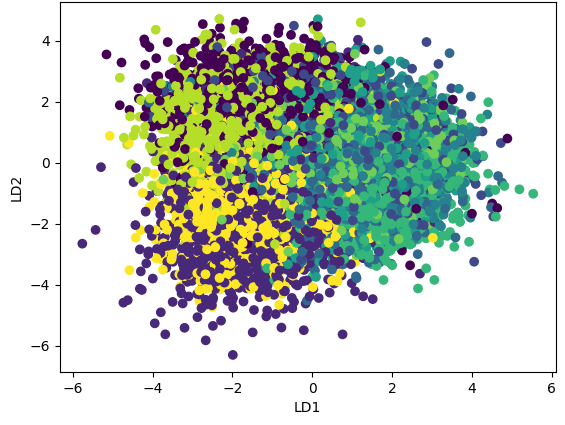
\includegraphics[width=\linewidth]{Figures/LDA.png} % Adjust width to \linewidth for full use of allocated space
  \captionsetup{font=scriptsize} % Change caption size
  \caption{Dataset projected with LDA}
  \label{fig:sub1}
\end{subfigure}% <-- Remove extra spaces here
\hfill % Add this to fill the space between subfigures
\begin{subfigure}{0.32\textwidth} % Adjust width as needed
  \centering
  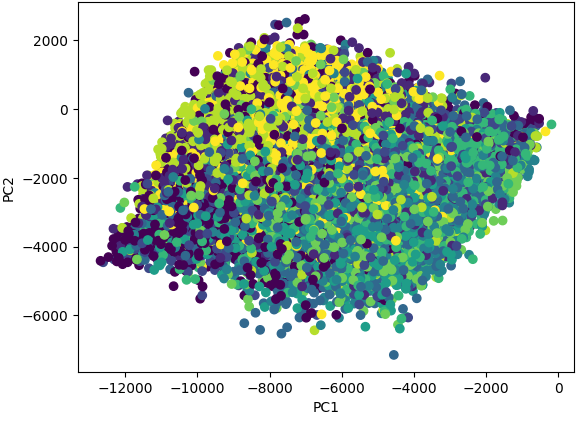
\includegraphics[width=\linewidth]{Figures/PCA.png}
  \captionsetup{font=scriptsize} % Change caption size
  \caption {Dataset projected with PCA}
  \label{fig:sub2}
\end{subfigure}
\hfill % Add this to fill the space between subfigures
\begin{subfigure}{0.305\textwidth} % Adjust width as needed
  \centering
  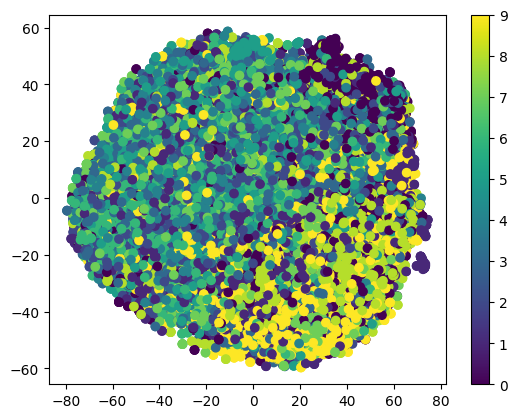
\includegraphics[width=\linewidth]{Figures/tsne.png}
  \captionsetup{font=scriptsize} % Change caption size
  \caption{Dataset projected with t-SNE}
  \label{fig:sub3}
\end{subfigure}
\caption{Projection of the dataset in different subspaces}
\label{fig:test}
\end{figure}
\noindent
Elucidating some differences, PCA preserves the variance in the data, whereas t-SNE preserves the relationships between data points in a lower-dimensional space, making it quite a good algorithm for visualizing complex high-dimensional data. 
\noindent
Due to LDA's discriminatory behavior, it projects the dataset into a 2-D subspace with some forms of clusters already visible. PCA technique projects the entire dataset into a 2-D subspace based on the direction of maximum variance. The t-SNE algorithm finds the similarity measure between pairs of instances in higher and lower dimensional space. After that, it tries to optimize two similarity measures. The optimization process allows the creation of clusters and sub-clusters of similar data points in the lower-dimensional space that are visualized to understand the structure and relationship in the higher-dimensional data.


 
\begin{figure}[h]
\centering
\begin{subfigure}{0.32\textwidth} % Adjust width as needed
  \centering
  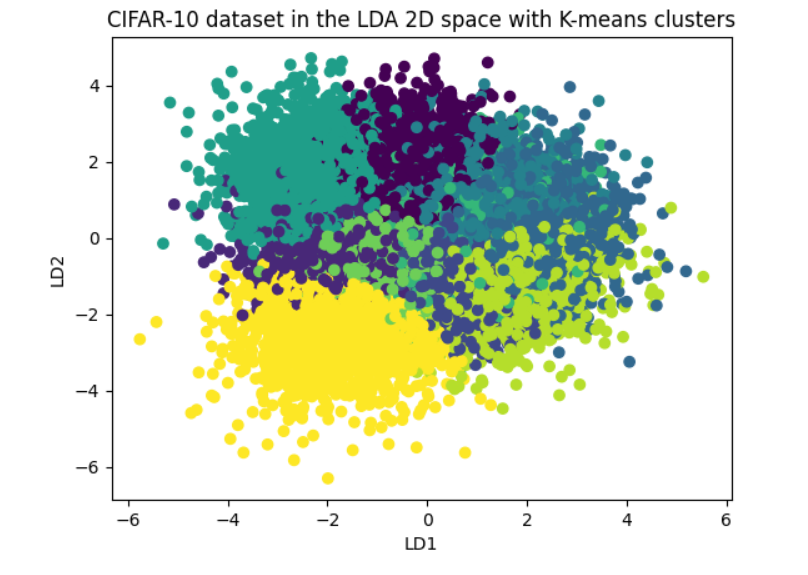
\includegraphics[width=\linewidth]{Figures/LDA+k-means.png} % Adjust width to \linewidth for full use of allocated space
  \captionsetup{font=scriptsize} % Change caption size
  \caption{K-Means + LDA}
  \label{fig:sub4}
\end{subfigure}% <-- Remove extra spaces here
\hfill % Add this to fill the space between subfigures
\begin{subfigure}{0.32\textwidth} % Adjust width as needed
  \centering
  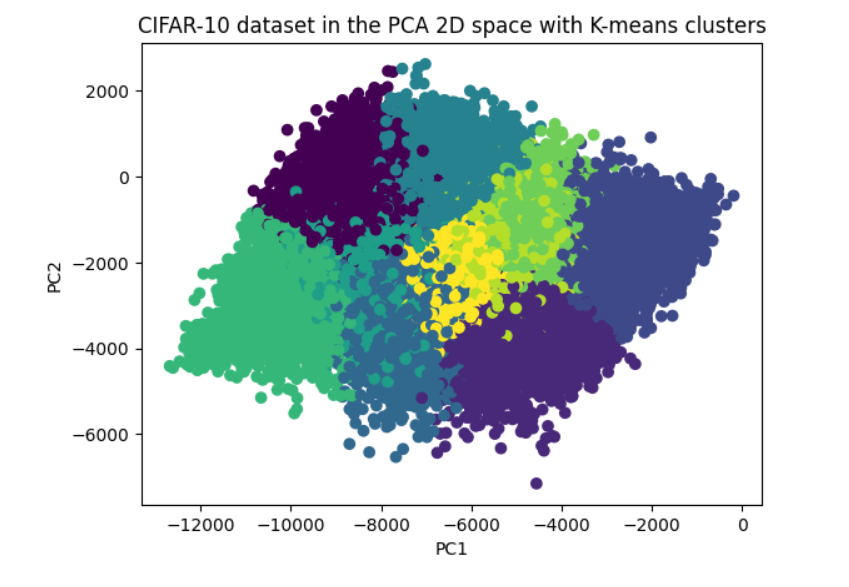
\includegraphics[width=\linewidth]{Figures/PCA+k-means.png}
  \captionsetup{font=scriptsize} % Change caption size
  \caption {K-Means + PCA}
  \label{fig:sub5}
\end{subfigure}
\hfill % Add this to fill the space between subfigures
\begin{subfigure}{0.305\textwidth} % Adjust width as needed
  \centering
  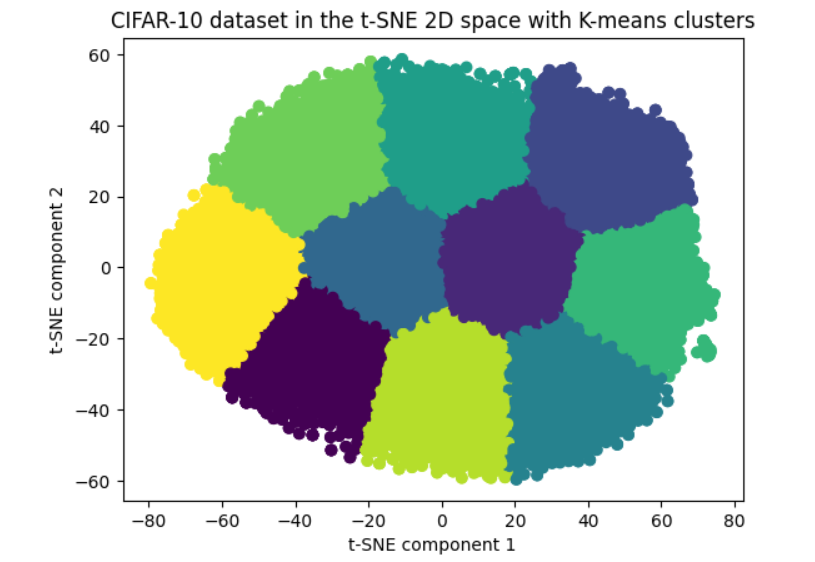
\includegraphics[width=\linewidth]{Figures/tsne+k-means.png}
  \captionsetup{font=scriptsize} % Change caption size
  \caption{K-Means + t-SNE}
  \label{fig:sub6}
\end{subfigure}
\caption{K-Means with various dimensionality reduction techniques}
\label{fig:test}
\end{figure}
\noindent
Using K-Means with n-clusters=10, we pass each of the unique transformed datasets through the K-Means algorithm. As seen from fig~\ref{fig:sub6}, t-SNE forms the best descriptive clusters. t-SNE converts similarities between data points into joint probabilities and minimizes the differences, thus better visualizing clusters. PCA in fig~\ref{fig:sub5} forms more compact and differentiable clusters than LDA based on the direction of maximum variability. Noticeably, each cluster is defined better (data points in a cluster do not separate much) using LDA since it minimizes the within-class scatter too. The degree of overlap between classes decreases on moving from LDA to PCA to t-SNE.

\newpage

\section {Other Approaches}
\subsection {Clustering using K-Means with Convolutional Neural Networks}
\noindent CNN features were extracted using a pre-trained VGG16 model. These features were passed on to the K-Means algorithm with the parameter of n-clusters set to 10.



\noindent To calculate the accuracy of this entire model, we had to perform more processing on the clusters given by K-Means. 
\noindent y-train and y-test already had inbuilt classes for each object. We aimed to assign those same numerical classes to the clusters predicted by this model.\newline 
\noindent Giving more context, Airplane is labelled as class '1'. The cluster '1' defined by this model should also correspond to only airplane images and not to automobile or bird images. The Hungarian algorithm (also known as the linear sum assignment) is used to find the best matching between clusters and true labels.
\newline \noindent The steps utilized are given below:
\begin{itemize}
    \item []\textbf{Calculate Cost Matrix}: The code calculates a confusion matrix, which represents the count of instances that are assigned to each cluster (rows) and each true label (columns).
\newline\noindent It iterates over each pair of cluster assignments and true labels, counting the number of instances that fall into that category.
    
    \item[] \textbf{Calculate Cost Matrix}:
  The cost matrix is created by taking the negative of the confusion matrix. This is because the Hungarian algorithm (used for assignment) seeks to minimize the total cost, so by using the negative of the confusion matrix, we can find the maximum assignment (which is equivalent to minimizing the negative assignment).

    \item []\textbf{Hungarian Algorithm (Linear Sum Assignment)}:
The Hungarian algorithm takes the cost matrix as input and returns the row and column indices that represent the best assignment.
            

    \item[] \textbf{Match Predicted Cluster Assignments to True Labels}:
  
The matching indices obtained from the Hungarian algorithm are used to match the predicted cluster assignments to the true labels.
\newline \noindent
This creates a new array \texttt{cluster\_assignments\_matched} where each element corresponds to the true label assigned to each instance.

    \item []\textbf{Calculate Accuracy}:

The accuracy is calculated by comparing the matched cluster assignments to the true labels y-test.
It calculates the proportion of correctly matched instances out of the total number of instances.
This model achieved an accuracy of about 22.3\%.

\end{itemize}
\newpage
\subsection {Classification using Fourier domain convolutions with ANN}
Convolutions capture underlying features in image data much better than linear layers. We use this concept of convolutions and our restriction of only being able to use simple Artificial Neural Networks to improvise and leverage the concept of Fourier Transforms to incorporate frequency domain convolutions. \newline 

\noindent The fast fourier transform function from PyTorch was used to obtain the frequency domain spectrum, out of which the high frequency components were picked which are known to correspond to edges and detailed textures.\newline 

\noindent This fact is of importance since most Machine Learning models we've implemented so far seem to be distracted by the colors in the images and other noise. The reduced frequency domain features were then used to train the simple neural network. \newline

\noindent The classification results were promising with as they were on par with our best approaches such as HOG combined with SVMs. \newline

\noindent These results could further be refined with hyperparameter tuning and other optimization techniques.
\subsection {Using Similarity function for retrieval}
\noindent
We also experimented with similarity functions such as cosine similarity.\newline 

\noindent  This experiment included setting up a pipeline from loading the data, extracting features using a pre-trained ResNet model, computing cosine similarity, and then displaying the most similar images by retrieving the images with the highest score. \newline

\noindent The results were less than favorable, since the similarity function seemed to focus on information such as colors in the images rather than identifying the objects and textures, though this could be attributed to the small image size and low resolution. Refer to fig~\ref{fig:sim}


% Define fonts for headings and subheadings
% \titleformat*{\section}{\Large\bfseries\sffamily}
% \titleformat*{\subsection}{\large\bfseries\sffamily}
 \begin{figure}
            \centering
            \includegraphics[width=0.77\linewidth]{Figures/cosine_similarity.png}
            \caption{Retrieval using cosine similarity}
            \label{fig:sim}
        \end{figure}


\newpage



\section {The Retriever Model}


\begin{itemize}
\item[] \textbf{Usage:} The functionality of our retriever model allows a user to pick one of the trained models available in the backend, along with a preprocessing method.
Upon clicking any of the images in the displayed ones, inference is performed by the chosen model and similar samples are retrieved based on the predictions of the model. The working is shown in figures~\ref{fig:r2} and~\ref{fig:r3}.



    
    \item[] \textbf{Implementation Details:} The Retriever’s implementation works as given in fig~\ref{fig:r1}
    
\begin{figure}[h]
\centering

  \centering
  \includegraphics[width=\linewidth]{Figures/retriever.png} % Adjust width to \linewidth for full use of allocated space
   % Change caption size
  \caption{UML of retriever}
  \label{fig:r1}
\end{figure}

    
    \item[] \textbf{Image Retriever:} A class was created that takes in the model, input image sample and preprocessing type as the inputs, and has the functionality to run inference and return similar images.
    
    \item[] \textbf{GUI:} GUI was made using PyQt5 and related functionality. The GUI displays a set of random clickable images, the user can then select an image to perform retrieval based on, and the retrieved images are displayed.
    
    \item[] \textbf{Data Handler:} A wrapper to make accessing data easier was created. The data is stored in the /docs/ directory in the repository.
    \newline
    
\begin{figure}[H]
\begin{subfigure}{0.4\textwidth} % Adjust width as needed
  \centering
  \includegraphics[width=\linewidth]{Figures/retriever model.png}
  \captionsetup{font=scriptsize} % Change caption size
  \caption {The retriever application}
  \label{fig:r2}
\end{subfigure}
\hfill % Add this to fill the space between subfigures
\begin{subfigure}{0.32\textwidth} % Adjust width as needed
  \centering
  \includegraphics[width=\linewidth]{Figures/retrieval.png}
  \captionsetup{font=scriptsize} % Change caption size
  \caption{Retrieval of similar images}
  \label{fig:r3}
\end{subfigure}
\caption{Retriever Model}
\label{fig:retrieverr}
\end{figure}
\end{itemize}

	\newpage
\section{Summary}
\label{sec:app}
The main objective of this project was to explore the possible classical Machine Learning solutions to the problem of Content-Based Image Retrieval. To that end, the project had been laid out into two different sections, the first stretch towards the mid-term mainly focused on solving the problem using Classification approaches. The second stretch was used to focus on carrying out experiments that leveraged the usage of Clustering-based techniques. Apart from using traditional Classification and Clustering techniques, certain other ideas were also experimented with such as using the idea of Fourier Domain Features incorporated into an Artificial Neural Network to emulate Convolutions, using the Clustering algorithm on features extracted from a pre-trained CNN model, and using a similarity function such as the cosine similarity to perform retrieval.

	


\appendix

\section{Contributions }
\label{sec:contribution}
\begin{enumerate}
\item Shyam: Ran experiments to benchmark models with no pre-processing on the dataset to create a demo code template others could use to run experiments. Implemented Fourier Domain Convolutions with ANN and similarity function retrieval. Implemented the retrieval pipeline. Prepared the project page and deployed the model. Prepared the video. Proofread and helped with the report. Led the team and distributed tasks..
\item Neermita: Ran experiments with PCA transformed data on various different classifiers. Implemented Clustering use K-Means with PCA, LDA and t-SNE transformed data. Took a shot at implementing clustering with CNNs. Prepared most of the report.
\item Siddhesh: Ran experiments with Hog extracted features on various different classifiers. Helped prepare the initial draft of the report.
\item Sakshi: Ran experiments with LDA extracted features on various different classifiers. 
\item Bhargavi: Ran experiments with SIFT extracted features on various different classifiers. Performed failure case analysis.
\end{enumerate}
\newpage





\bibliography{refs}	
	
\end{document}

